\documentclass{article}
\usepackage[paperwidth=5.5in, paperheight=8.5in, twoside, margin=0.8in]{geometry}
\usepackage{graphicx}
\begin{document}
\author{James Babcock (jimrandomh@gmail.com)}
\title{Petrov Day}

% Ideas to incorporate:
%    Move the Malthus bit to after three candles are lit (establishing the pattern)
%    Incorporate a tree of extinct human relatives, in the section about evolution
%    Mention collapsed civilizations: Easter Island, that island hypothesized as being Atlantis, Mayans, etc
%    Work in a mention of Moloch
%    Discuss the post-WW2 measures as a way of ending on a positive note: formation of the UN, twinning, reaties
%    Mention abandonment of nuclear powered rockets
%    Mention environmental successes

% Through the years her work continued to yield surprising insights, such as
% the unsettling discovery that chimpanzees engage in primitive and brutal
% warfare. In early 1974, a “four-year war” began at Gombe, the first record
% of long-term “warfare” in nonhuman primates. Members of the Kasakela group
% systematically annihilated members of the “Kahama” splinter group. --Jane Goodall

% Most species do their own evolving, making it up as they go along, which is
% the way Nature intended. -–Terry Pratchett

% Most gods throw dice, but Fate plays chess, and you don’t find out til too
% late that he’s been playing with two queens all along. -–Terry Pratchett

% Man still bears in his bodily frame the indelible stamp of his lowly origin. –Charles Darwin


\newcommand{\divider}{ %{{{
	% From http://tex.stackexchange.com/questions/32711/totally-sweet-horizontal-rules-in-latex
	\nointerlineskip \vspace{\baselineskip}
	\hspace{\fill}\rule{0.5\linewidth}{.7pt}\hspace{\fill}
	\par\nointerlineskip \vspace{\baselineskip}
} %}}}
\newcommand{\stagedir} [1] { %{{{
	\begin{itshape}
	#1
	\end{itshape}
} %}}}
\newcommand{\blockquote} [2] { %{{{
	\begin{center}
		\parbox{3.5in}{
			``#1''
			\begin{flushright}
				--- #2
			\end{flushright}
		}
	\end{center}
} %}}}
\newcommand{\blockquoteUnattributed} [1] { %{{{
	\begin{center}
		\parbox{3.5in}{
			``#1''
		}
	\end{center}
} %}}}
\newcommand{\blockquoteUnmarked} [2] { %{{{
	\begin{center}
		\parbox{3.5in}{
			#1
			\begin{flushright}
				--- #2
			\end{flushright}
		}
	\end{center}
} %}}}
\newcommand{\poem} [2] { %{{{
	\begin{center}
		\parbox{3.5in}{
			#1
			\begin{flushright}
				--- #2
			\end{flushright}
		}
	\end{center}
} %}}}
\newcommand{\page} [1] { %{{{
	\divider
	#1
	\divider
	\newpage
} %}}}
\newcommand{\sidePage} [1] { %{{{
	#1
	\newpage
} %}}}

% Don't indent paragraphs
\setlength{\parindent}{0cm}

\setlength{\parskip}{\baselineskip}

%%%%%%%%%%%%%%%%%%%%%%%%%%%%%%%%%%%%%%%%%%%%%%%%%%%%%%%%%%%%%%%%%%%%%%

% Front Matter
% Title page {{{
Petrov Day

September 26
\newpage
% }}}

% Introduction Section
% Light candle 1
% Intro page {{{
\page{

\stagedir{Content warning: Engineered to evoke strong feelings of existential terror.}

\stagedir{Stage directions are written in italics, like this. All other text is
to be read aloud. Whenever there is a horizontal line, it becomes the next
person's turn to speak, going clockwise.}

This day, September 26, is Petrov Day. In 1983, the story of humanity nearly
ended. We're gathered here to remember that moment, and others like it. But to
really feel the magnitude of those events, we need to visit them in their
proper context. Let us begin the story of human history, starting from the
beginning.

\divider

\blockquote{In the beginning, the universe was created. This has made a lot of
people very angry, and been widely regarded as a bad move.}{Douglas Adams}

\divider

Ok, fast forward over the thirteen billion year long prequel. Our story begins
in the age of myth, of fossils and legends. It starts with the invention of fire.

} %}}}
% Prometheus quote {{{
\sidePage{
\blockquote{I've hunted down and stolen, inside the hollow of a fennel's stalk,
the seed of fire, a gift that has proven itself to be the teacher of every craft
and the greatest resource for humans.  Such is the crime I have committed and
this is the penalty I am to suffer: nailed and chained on this rock beneath the
open sky.}{Prometheus Bound}

% TODO: Picture of a candelabrum with one candle placed and lit

\stagedir{Light the left-most candle, to represent the invention of fire. Point
out the location of the nearest fire extinguisher, then turn off all other lights in
the room.}
} %}}}

% Prehistory

% About Fire {{{
\page {

Depending which archaeologists you ask, fire was first used by either Homo
Erectus of Homo Ergaster, some time between 400 thousand and 1.7 million years
ago. Cooking is believed to have enabled larger, more energy-intensive brains,
allowing the evolution of increased intelligence, and language.

\divider

\blockquote{Most species do their own evolving, making it up as they go along,
which is the way Nature intended. And this is all very natural and organic and
in tune with mysterious cycles of the cosmos, which believes that there's
nothing like millions of years of really frustrating trial and error to give a
species moral fiber and, in some cases, backbone.}{Terry Pratchett}

} %}}}
% Family tree {{{
\sidePage {
\stagedir{TODO: Insert picture of genus homo tree here, with Homo Sapiens
represented by a drawing, and all other variants represented by captioned
pictures of their skulls}
} %}}}
% CUT: Fire and speech {{{
%\page {
%
%Estimates place the invention of fire somewhere from 400,000 to 1.7 million
%years ago, while anatomically modern humans did not appear until 200,000 years
%ago.
%
%Fire is not, by itself, of particularly great importance. It grants protection
%from the cold of winter, and access to foods that would otherwise be inedible;
%but if it had stopped there, then the story of genus homo would have been
%unremarkable. But fire enabled, and favored, creatures with larger brains, and
%some time after that - we don't know when - our ancestors began to speak.
%
%} % }}}
% The invention of language: Candle 2 {{{
\page{

\blockquote{It's perfectly obvious that there is some genetic factor that
distinguishes humans from other animals and that it is language-specific. The
theory of that genetic component, whatever it turns out to be, is what is
called universal grammar.}{Noam Chomsky}
% Source: http://www.slate.com/articles/health_and_science/new_scientist/2012/03/noam_chomsky_on_linguistics_and_climate_change_.html

%\blockquote{It certainly is not a true instinct, for every language has to be learnt. It
%differs, however, widely from all ordinary arts, for man has an instinctive
%tendency to speak, as we see in the babble of our young children; whilst no
%child has an instinctive tendency to brew, bake, or write.}{Charles Darwin,
%Descent of Man (1871)}

}

\sidePage {

% TODO: Picture of the candelabrum with two candles lit

\stagedir{Take the first candle, which represents the invention of fire. Use it
to light the second candle, which represents the evolution of language.}

\stagedir{Pass the candle around the circle. When you hold the candle, it is
your turn to speak. What is your name, and when (what year) is your earliest
memory?}

}
% }}}
% Agriculture: Candle 3 {{{
\page{

Language is the first key to technology; with it, early humans could accumulate
knowledge, not just in genes, but also in sayings and traditions.

They gave names to people around them. They gave names to species of animals
and plants. They gave names to actions and to places and to strategies. They
called some of these good, and called some of them bad. They learned to share
their knowledge, and they learned to deceive each other. They built families
and communities.

They began the long, slow process of taming the wilderness. Their tribes grew
to cities. What became of them?

}

\sidePage {

\stagedir{Take the second candle, which represents language. Use it to light
the third candle, which represents agriculture.}

\stagedir{Then, everyone sing together:}

\poem{
	Hands chip the flint, light the fire, skin the kill\newline
	Feet move the tribe track the herd with a will\newline
	Mankind struggles in the cellar of history\newline
	Time to settle down, time to grow, time to breed\newline
	\newline
	Plow tills the soil, plants the seed, pray for rain\newline
	Scythe reaps the wheat, to the mill, to grind the grain\newline
	Towns and cities spread to empire overnight\newline
	Hands keep building as we chant the ancient rite}{Uplift by Andrew Eigel}

% TODO: Picture of the candelabrum with three candles lit

}
% }}}
% The Malthusian Trap {{{

\page {
\blockquote{The power of population is so superior to the power of the earth to
produce subsistence for man, that premature death must in some shape or other
visit the human race. The vices of mankind are active and able ministers of
depopulation.  They are the precursors in the great army of destruction, and
often finish the dreadful work themselves. But should they fail in this war of
extermination, sickly seasons, epidemics, pestilence, and plague advance in
terrific array, and sweep off their thousands and tens of thousands. Should
success be still incomplete, gigantic inevitable famine stalks in the rear, and
with one mighty blow levels the population with the food of the
world.}{Thomas Malthus (1798)}
}

\sidePage {

%Mankind lived in equilibrium between growth and collapse, between knowledge
%gained and knowledge forgotten. In that world, stories last only a few
%generations. For two hundred thousand years, nothing but genes survived.

% TODO: Picture of the candelabrum

\stagedir{Take the third candle, which represents agricultural society. Pass it
around the circle.

Blow it out. Then return it to its place in the candelabrum.}

}
% }}}
% Agriculture {{{
\page{

But that was enough. Some ten thousand years ago, humans began the process of
domestication. Rather than hunt and forage, they would seize control of nature,
plant fields of things to eat, select the best and bring about abundance. The
world got easier.

This raised the population density, but the Malthusian limit soon caught up.
The equilibrium between growth and starvation was not broken. Worse, farming
brought bad diets, poor health, and numerous social ills.

\divider

\blockquote{Archaeologists studying the rise of farming have reconstructed a crucial stage
at which we made the worst mistake in human history. Forced to choose between
limiting population or trying to increase food production, we chose the latter
and ended up with starvation, warfare, and tyranny.}{Jared Diamond (1987)}

\divider

Despite its problems, farming enabled the growth of civilizations, and the
rulers of some of these civilizations came to realize that they did not want to
be forgotten. Some built monuments. About 5,000 years ago, some began to write.

The equilibrium between learning and forgetting was finally broken.

Of that age, what memories remain?

}
%}}}

% History

% Invention of writing: Candle 3 again; write names of family members {{{
\page{
\stagedir{Using the second candle, which represents language, relight the third
candle to represent the invention of writing.

Then, everyone read this passage silently.}

\poem{
	I met a traveller from an antique land\newline
	Who said: Two vast and trunkless legs of stone\newline
	Stand in the desert. Near them, on the sand,\newline
	Half sunk, a shattered visage lies, whose frown,\newline
	And wrinkled lip, and sneer of cold command,\newline
	Tell that its sculptor well those passions read\newline
	Which yet survive, stamped on these lifeless things,\newline
	The hand that mocked them and the heart that fed:\newline
	And on the pedestal these words appear:\newline
	"My name is Ozymandias, king of kings:\newline
	Look on my works, ye Mighty, and despair!"\newline
	Nothing beside remains. Round the decay\newline
	Of that colossal wreck, boundless and bare\newline
	The lone and level sands stretch far away}{Percy Bysshe Shelley (1818)}

\stagedir{When you have finished reading, take a piece of paper and write down
the name of the oldest family member - living or dead - that you can identify.

When everyone has written something, continue to the next page.}

}
% }}}
% Writing and The Rosetta Stone {{{
\page{

We know more about what the world was like after people started writing, but
not very much survived. One of the most important writings was discovered by
French soldiers in the wall of Fort Julien: the Rosetta Stone, important
because it was written in three languages, two previously untranslatable. After
a long string of honorifics and decrees about taxes and succession, it
declares: there shall be a new holiday!

\divider

\blockquote{On these days in every month, on which there shall be sacrifices
and libations and all the ceremonies customary at the other festivals, and the
offerings shall be given to the priests who serve in the temples. And a festival
shall be kept for King Ptolemy, the Ever-Living, the Beloved of Ptah, the God
Epiphanes Eucharistos, yearly in the temples throughout the land from the 1st
of Thoth for five days ... This decree shall be inscribed on a stela of hard
stone in hieroglyphic and demotic and Greek characters and set up in each of the
first, second, and third temples beside the image of the ever living
king.}{The Rosetta Stone, ca. 196 BC}

}

\sidePage{

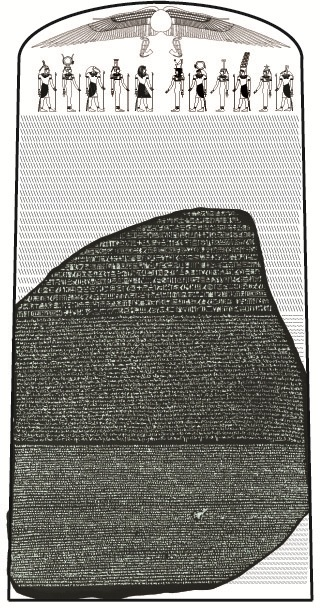
\includegraphics[width=3in]{RosettaStone.jpg}

}
% }}}
% Scientific Method: Candle 4; write something surprising you learned {{{
\page{

% TODO: Rewrite this paragraph to instead talk about early known examples of
% written mathematics.

The majority of writing consisted of geneologies, legal codes, and fastastic
stories. But some writing represented progress in philosophy and mathematics,
eventually culminating in the invention of the scientific method.

\divider

\blockquote{Mathematics is the gate and key of the sciences... Neglect of
mathematics works injury to all knowledge, since he who is ignorant of it
cannot know the other sciences or the things of this world. And what is worse,
men who are thus Ignorant are unable to perceive their own ignorance and so do
not seek a remedy.}{Roger Bacon, Opus Majus (1266)}
}
\sidePage{

\stagedir{
Using the third candle, which represents writing, light the fourth candle to
represent the scientific method.

% TODO: Picture of the candelabrum with three candles lit

% TODO: Replace this with a better written thing
Then, everyone write down something surprising they learned about the
world, and put it in the middle. When everyone has written something, continue
to the next page.}

}
% }}}
% Black Death: Blow out candle 4 {{{
\page{

The scientific method, combined with writing and a university system, marked
the start of an accumulation of knowledge. This could have marked the beginning
of a slow transition into the modern era. Instead, 81 years later, history was
derailed by a great plague.

}
\page{

\stagedir{Take the fourth candle, which represents the progress of science.
Hold it, while you read the quote.}

\blockquote{The seventh year after it began, it came to England and first began
in the towns and ports joining on the seacoasts, in Dorsetshire, where, as in
other counties, it made the country quite void of inhabitants so that there
were almost none left alive. ... But at length it came to Gloucester, yea even
to Oxford and to London, and finally it spread over all England and so wasted
the people that scarce the tenth person of any sort was left alive.}{Geoffrey
the Baker, Chronicon Angliae (1360)}

\stagedir{Blow out the candle. Then return it to its place on the candelabrum.}

} %}}}
% Printing press: Re-light candle 4 {{{
\page{

% TODO: Rewrite this, it has the wrong tone
%Our knowledge grew by leaps and bounds, but once gained, it spread slowly. Deep
%knowledge required books, and books were written by hand, painstakingly copied
%in a process that could take years. They were so rare that most humans were
%illiterate--why learn to read, if you'll never have the chance?
%
%Progress, and accumulated knowledge, was the domain of an elite few, and was
%often lost; for scrolls rot, books burn and oral traditions tell only so much.
%Billions lived and died without ever grasping the accumulated knowledge of
%humanity.
%
%Then around 1439, Johannes Gutenberg invented the movable-type printing press.
%At first, there was only one book printed; but it sparked widespread literacy,
%and expanded the intellectual class from a tiny minority to a small one.

The plague killed about half the population of Europe died during a four-year
period, and it recurred repeatedly throughout the next three centuries killing
double-digit percentages of the population each time. Between plagues, wars,
and famines, there was little time to build or preserve knowledge.

Preserving knowledge required redundancy. In 1439, Gutenberg gave it that.

\divider

\blockquoteUnmarked{``Pray, friend Martin, how many impressions can be made by
this press in a day?'' ``About three hundred, if we work it constantly.'' ``Is
it possible!'' exclaimed Peter. ``Now indeed will books multiply. What will the
plodding copyists say to this?''}{Emily Clemens Pearson, Gutenberg and the Art
of Printing (1870)}
}

\page{

\stagedir{Take the fourth candle, which represents the progress of science.

Touch it to each of the other three candles in turn, until it is lit. Then
return it to its place on the candelabrum.}

} % }}}

% Age of Progress

% Progress of Science {{{
\page{

\stagedir{Take the fourth candle, which represents science. Hold it, while you
read the quote, then pass it directly to the next person.}

\blockquote{By the aid of a telescope any one may behold this in a manner which so
distinctly appeals to the senses that all the disputes which have tormented
philosophers through so many ages are exploded at once by the indisputable
evidence of our eyes, and we are freed from wordy disputes upon this subject,
for the Galaxy is nothing else but a mass of innumerable stars planted together
in clusters. Upon whatever part of it you direct the telescope straightway a
vast crowd of stars presents itself to view; many of them are tolerably large
and extremely bright, but the number of small ones is quite beyond
determination.}{Galileo, The Starry Messenger (1610)}
% Footnote: Some words have been modernized. Sidereal->Starry, irrefragable->indisputable.

\divider

\blockquote{By calculations similar to these may be determined universally, what
expectations are warranted by any experiments, according to the different number
of times in which they have succeeded and failed; or what should be thought of
the probability that any particular cause in nature, with which we have any
acquaintance, will or will not, in any single trial, produce an effect that has
been conjoined with it.}{Rev. Thomas Bayes, An Essay towards solving a Problem
in the Doctrine of Chances (1763)}

}

\page{

\blockquote{I saw in a dream a table where all elements fell into place as
required. Awakening, I immediately wrote it down on a piece of paper, only in
one place did a correction later seem necessary.}{Dmitri Mendeleev (1864)}

\divider

\blockquote{I speak without exaggeration when I say that I have constructed
3,000 different theories in connection with the electric light, each one of
them reasonable and apparently likely to be true. Yet only in two cases did my
experiments prove the truth of my theory. My chief difficulty was in
constructing the carbon filament. ... Every quarter of the globe was ransacked
by my agents, and all sorts of the queerest materials used, until finally the
shred of bamboo, now utilized by us, was settled upon.}{Thomas Edison (1890)}

} %}}}

% Astronomy {{{
\page{

% TODO: Rewrite this, it has the wrong tone
With printed books, mysteries, once solved, could \textit{stay} solved; and once
invented, a device could \textit{stay} invented. And so, less gradually than
before, the universe started getting less mysterious--starting with the night sky.

\divider

\blockquote{By the aid of a telescope any one may behold this in a manner which so
distinctly appeals to the senses that all the disputes which have tormented
philosophers through so many ages are exploded at once by the indisputable
evidence of our eyes, and we are freed from wordy disputes upon this subject,
for the Galaxy is nothing else but a mass of innumerable stars planted together
in clusters. Upon whatever part of it you direct the telescope straightway a
vast crowd of stars presents itself to view; many of them are tolerably large
and extremely bright, but the number of small ones is quite beyond
determination.}{Galileo, The Starry Messenger (1610)}
% Footnote: Some words have been modernized. Sidereal->Starry, irrefragable->indisputable.

} %}}}
% Mechanics, Statistics{{{
\page{

Isaac Newton, the inventor of calculus and classical mechanics, refined
Galileo's experimental method, and formulated four universal principles of
scientific reasoning that remain relevant today:

\blockquote{Matters that vexed the minds of ancient seers, And for our learned doctors
often led to loud and vain contention, now are seen In reason's light, the
clouds of ignorance Dispelled at last by science. Those on whom Delusion cast
its gloomy pall of doubt, Upborne now on the wings that genius lends, May
penetrate the mansions of the gods And scale the heights of heaven. O mortal
men, Arise! And, casting off your earthly cares, Learn ye the potency of
heaven-born mind, Its thought and life far from the herd withdrawn!}{Edmund Halley, preface to Newton's Principia Mathematica (1687)}

\divider

Some time around 1760, Thomas Bayes wrote what we now call Bayes Theorem. It
remained unpublished among his papers until Richard Price found it, two years
after his death, in 1763.

\blockquote{By calculations similar to these may be determined universally, what
expectations are warranted by any experiments, according to the different number
of times in which they have succeeded and failed; or what should be thought of
the probability that any particular cause in nature, with which we have any
acquaintance, will or will not, in any single trial, produce an effect that has
been conjoined with it.}{Rev. Thomas Bayes, An Essay towards solving a Problem
in the Doctrine of Chances (1763)}

%The most ancient humans thought lightning was the tool of the gods, and they
%were not far wrong. When we mastered the secrets of electricity, we gained
%power beyond anything a mere thunder god could dream. We harnessed rivers, we
%burned the bones of forgotten beasts, for the energy to turn night into day.

} % }}}

% Industrial era

% Industrialization: Candle 5; write something you created {{{
\page{

Piece by piece, discoveries and technologies fell into place, each one making
life slightly easier, and pushing our ignorance slightly back.

\blockquote{I speak without exaggeration when I say that I have constructed
3,000 different theories in connection with the electric light, each one of
them reasonable and apparently likely to be true. Yet only in two cases did my
experiments prove the truth of my theory. My chief difficulty was in
constructing the carbon filament. ... Every quarter of the globe was ransacked
by my agents, and all sorts of the queerest materials used, until finally the
shred of bamboo, now utilized by us, was settled upon.}{Thomas Edison (1890)}

\stagedir{Using the fourth candle, which represents the scientific method,
light the fifth candle to represent industrialization.

Then, each person writes down something they've created, and puts it in the
middle.}

} % }}}
% Industrialization {{{
\page{

With reason and learning, with lightning and steel, humans built on a scale
never before seen. As we created tools and infrastructure, small gains in
efficiency compounded, and compounded, and compounded again, leading to yet
better tools and yet more infrastructure. We built tractors that feed cities,
railroads that span continents, and economies that coordinate thousands of
millions of humans.

\blockquote{If a device would save in time just 10 per cent. or increase results 10 per
cent., then its absence is always a 10 per cent. tax. If the time of a person
is worth fifty cents an hour, a 10 per cent. saving is worth five cents an
hour. If the owner of a skyscraper could increase his income 10 per cent., he
would willingly pay half the increase just to know how. The reason why he owns
a skyscraper is that science has proved that certain materials, used in a given
way, can save space and increase rental incomes. A building thirty stories high
needs no more ground space than one five stories high. Getting along with the
old-style architecture costs the five-story man the income of twenty-five
floors. Save ten steps a day for each of twelve thousand employees and you will
have saved fifty miles of wasted motion and misspent energy. Those are the
principles on which the production of my plant was built up.}{Henry Ford, "My Life and Work" (1922)}

\divider

As we enter the thirties and forties, many of the rules on which human society
was built have given way to science and industry. Prior to this point,
technological progress moved at the speed of civilization, and its effects were
mainly effects on societies. Each technology has a name attached, but those
names do not matter much.

} % }}}
% Political Science {{{
\page{
% Sneaky quote
\blockquoteUnattributed{Those material inventions, beginning with the use of stones as
weapons, which led to the domestication of animals, the production of fire by
artificial means, down to the marvellous inventions of our own days, show
clearly that an individual was the originator in each case. The nearer we come
to our own time and the more important and revolutionary the inventions become,
the more clearly do we recognize the truth of that statement. All the material
inventions which we see around us have been produced by the creative powers and
capabilities of individuals.}

\divider

In 1687, Isaac Newton figured out calculus and mechanics, becoming master of
nothing. In 1890, Edison figured out how to practically apply electricity,
becoming master of a large business.

In 1939, someone figured out power - what we would now call political science.
And this time, it matters a great deal who he was. He was the writer of the
last quote. And he is now widely considered the most evil man ever to have
lived - because of the war he started, his goal, and his methods.

} % }}}
% World War 2 {{{
\page{

\blockquote{I should like to call attention to the fact that the principle of
parliamentarian democracy, whereby decisions are enacted through the majority
vote, has not always ruled the world. On the contrary, we find it prevalent
only during short periods of history, and those have always been periods of
decline in nations and States.}{Adolf Hitler, Mein Kampf (1926)}

\divider

Starting in 1939 and continuing until 1945, World War 2 killed 2.5\% of the
world's population. Had it gone differently, it's likely that the entire world
would have fallen under a single totalitarian regime. This would not have meant
human extinction, exactly - but it would most likely mean the loss of
humanity's potential.

\divider

And so the physicists of the Manhattan Project created the atomic bomb - a
weapon to destroy entire cities, or the whole world. They did it, not because
they wanted it to exist, but because they believed the alternative was even
worse.

} %}}}
% Manhattan Project: Take candle 5, and drip wax. Light candle 6, the Atom {{{
\page{

\blockquote{Despite the vision and farseeing wisdom of our wartime heads of state, the
physicists have felt the peculiarly intimate responsibility for suggesting, for
supporting, and in the end, in large measure, for achieving the realization of
atomic weapons. Nor can we forget that these weapons as they were in fact used
dramatized so mercilessly the inhumanity and evil of modern war. In some sort
of crude sense which no vulgarity, no humor, no overstatement can quite
extinguish, the physicists have known sin; and this is a knowledge which they
cannot lose.}{Robert J. Oppenheimer (1947)}

\stagedir{Take the fifth candle, which represents industrialization. Hold it
over the stack of papers until three drops of wax fall. 

Then use it to light the sixth candle, which represents mastery of the atom.}

} % }}}
% Postwar Progress {{{
\page{

After the war, things settled down - but the pace of progress continued.

In 1951, the transistor.\newline
In 1952, the first model of action potentials in neurons.\newline
In 1953, the discovery of DNA's structure.\newline
In 1954, polypropylene plastic.\newline
In 1955, the Polio vaccine.\newline
In 1956, the first commercial nuclear power station.\newline
In 1957, Sputnik, the first orbital space flight.\newline
In 1958, the first prototype integrated circuit.\newline
In 1959, the alkaline battery.

\divider

But one thing we did \textit{not} invent, was artificial intelligence. In this
context of breathtaking progress, the Dartmouth Conference was held to study
the problem of artificial intelligence. Held two years before the first
prototype integrated circuit and 15 years before the first commercial
microprocessor, it would later come to symbolize wild over-optimism in the
field of AI.

} % }}}
% Dartmouth Conference 1956 {{{
\page{

\blockquote{We propose that a 2 month, 10 man study of artificial intelligence
be carried out during the summer of 1956 at Dartmouth College in Hanover, New
Hampshire.  The study is to proceed on the basis of the conjecture that every
aspect of learning or any other feature of intelligence can in principle be so
precisely described that a machine can be made to simulate it. An attempt will
be made to find how to make machines use language, form abstractions and
concepts, solve kinds of problems now reserved for humans, and improve
themselves. We think that a significant advance can be made in one or more of
these problems if a carefully selected group of scientists work on it together
for a summer.}{McCarthy et al, 1956}

} % }}}
% SETI 1961, Drake equation {{{
\page{

In 1961, the Search for Extraterrestrial Intelligence (SETI) held its first
conference at the National Radio Astronomy Observatory in West Virginia, to
discuss what is now called the Drake Equation:

\blockquote{I wrote down all the things you needed to know to predict how hard it's going
to be to detect extraterrestrial life. And looking at them it became pretty
evident that if you multiplied all these together, you got a number, N, which
is the number of detectable civilizations in our galaxy.}{Frank Drake}

In forty-odd years of searching, we have found no extraterrestrial life. Our
best estimates for the Drake equation, however, suggest that there should be.
This is the Fermi Paradox: where is everybody?

} % }}}
% Great Filter {{{
\page{

\blockquote{Humanity seems to have a bright future, i.e., a non-trivial chance
of expanding to fill the universe with lasting life. But the fact that space
near us seems dead now tells us that any given piece of dead matter faces an
astronomically low chance of begating such a future. There thus exists a great
filter between death and expanding lasting life, and humanity faces the ominous
question: how far along this filter are we?

Combining standard stories of biologists, astronomers, physicists,
and social scientists would lead us to expect a much smaller filter than we
observe. Thus one of these stories must be wrong. To find out who is wrong, and
to inform our choices, we should study and reconsider all these areas. For
example, we should seek evidence of extraterrestrials, such as via signals,
fossils, or astronomy.  But contrary to common expectations, evidence of
extraterrestrials is likely bad (though valuable) news. The easier it was for
life to evolve to our stage, the bleaker our future chances probably
are.}{Robin Hanson (1998)}

\divider

The absence of observed alien life, taken together with our current best
estimates of how unlikely it was for life to arise and to advance to the point
where we are now, means that there must be some filter further in our future,
which prevents most life from spreading through the stars. Therefore, either
our model of the past or of the universe is very substantially wrong, or there
is an obstacle in our future which most intelligent civilizations fail to pass.
We have several ideas about what that obstacle might be.

} % }}}
% Cuban Missile Crisis 1962: Drip wax {{{
\page{
In 1962, the cold war between the United States and the Soviet Union reached a
crisis. US destroyers under orders to enforce a naval quarantine off Cuba did
not know that the submarines the Soviets had sent to protect their ships were
carrying nuclear weapons. So the Americans began firing depth charges to force
the submarines to the surface, a move the Soviets interpreted as the start of
World War III.

\blockquote{We're going to blast them now! We will die, but we will sink them
all. We will not  disgrace our navy,}{Captain Valentin Grigorievitch Savitsky}

\stagedir{Take the sixth candle, which represents the atom, and hold it over
the stack of papers until three drops of wax fall.}

} % }}}
% Arkhipov {{{
\page {
That co-officer was Vasili Arkhipov. The launch of the submarine's nuclear
torpedo required the consent of all three senior officers aboard. Arkhipov was
alone in refusing permission, insisting the submarine surface to receive orders
from Moscow. Had he chosen differently, the likely result would have been
all-out nuclear war.

\divider

Meanwhile, technology marched on. And for the first time, it seemed that
technological progress might not go on forever, but build towards an ultimate
conclusion.

} % }}}
% 1963: IJ Good, Superintelligence: Place an unlit candle in the last spot {{{
\page{

\blockquote{Let an ultraintelligent machine be defined as a machine that can far surpass
all the intellectual activities of any man however clever. Since the design of
machines is one of these intellectual activities, an ultra-intelligent machine
could design even better machines; there would then unquestionably be an
"intelligence explosion," and the intelligence of man would be left far behind.
Thus the first ultraintelligent machine is the last invention that man need
ever make, provided that the machine is docile enough to tell us how to keep it
under control.}{I.J. Good, Speculations Concerning the First Ultraintelligent Machine (1963)}

\stagedir{Place an unlit candle in the last spot, to represent artificial
intelligence.}

} % }}}
% Moore's Law 1965: Light candle 7, Computers {{{
\page{

Two years later, Gordon Moore famously observed:

\blockquote{The complexity for minimum component costs has increased at a rate
of roughly a factor of two per year. Certainly over the short term this rate
can be expected to continue, if not to increase. Over the longer term, the rate
of increase is a bit more uncertain, although there is no reason to believe it
will not remain nearly constant for at least 10 years. That means by 1975, the
number of components per integrated circuit for minimum cost will be 65,000.}{Gordon Moore, 1965}

\stagedir{Using the fifth candle, which represents industrialization, light the
seventh candle to represent the invention of computers.}

Moore's Law has been rephrased many times, to talk about slightly different
things - clock rate, computation speed, cost per computation speed, cost per
computation. Some of these phrasings must eventually face fundamental physical
limits - but some of them need not. For now, the speed of computation is
increasing at the slightly slower rate of roughly a factor of two every other
year. It shows no sign of stopping.

} % }}}
% Space Travel {{{
\page{

Meanwhile, the rockets that had first been developed for war were turned to
exploration as well:

\blockquote{Here men from the planet Earth first set foot upon the Moon July
1969, A.D.  We came in peace for all mankind}{Apollo 11 Plaque}

Humans visited the moon five more times, the last in 1972. We have already left
Earth, and we have the potential to go further still. This small step has
inspired hope that we will one day travel to the stars, where there is space
enough for a billion billion humans to thrive.

} % }}}
% AI Winter {{{
\page{

Compared to landing on the moon, computers were just not that impressive. In
1973 the British Science Research Council commissioned James Lighthill to
evaluate the state of artificial intelligence:

\blockquote{Most workers in AI research and in related fields confess to a
pronounced feeling of disappointment in what has been achieved in the past
twenty-five years. Workers entered the field around 1950, and even around 1960,
with high hopes that are very far from having been realized in 1972. In no part
of the field have the discoveries made so far produced the major impact that
was then promised.}{James Lighthill, 1973}

\divider

So began the AI winter: a period of pessimism, reduced funding, and minimal
progress. We now know that AI is hard; how hard exactly, we don't know. Since
then, Moore's Law has continued - and so, every year, the difficulty drops a
little bit.

} % }}}
% Flynn Effect {{{
\page{
At this point, it's worth noting another effect, something like Moore's Law,
which also continues year after year: the Flynn effect. Ever since mental tests
were introduced, the mean IQ of Americans has been rising at a rate of about .3
points per year. I went to James Flynn's paper on this, published in 1984,
expecting to find a discussion of advancing intelligence, pick out an
illustrative quote and move on. That is not what I found.

While technology changes rapidly, it is often said that human nature doesn't
change. Rising IQs are a change to human nature, but a comprehensible one; it
is mostly a matter of the average people becoming more like the best people.
But human nature changes in more ways than one, and while Flynn was interested
in rising IQ test results, his goal was to reconcile them with falling scores
on a different test, the Scholastic Aptitude Test or SAT.

\divider

\blockquote{Our analysis dictates the conclusion that American 18-year-olds have
deteriorated .48 to .96 SDU in terms of a total package consisting of
motivation, study habits, self-discipline, and acquired verbal and writing
skills. Which is to say that only the upper, 17\% to 32\% of today's 18-year-olds
can match the upper half of young people as recently as 1963! The calculations
above should not be taken literally of course: They are merely meant to show
that if both IQ gains and SAT losses are taken to be real, rather than
artifacts of sampling error, then the deterioration of non-IQ personal traits
among young Americans must have been very great.}{James R. Flynn (1984)}

\divider

I don't know how to compare the personality traits of populations over time,
but I do know this: the world is suddenly filled with stressors and drugs and
superstimuli that enable humans to go insane in a variety of novel and exciting
ways, and we keep inventing new ones. Sometimes, humans go insane in ways that
are dangerous to those around them, and sometimes they go insane from positions
of power.

} % }}}
% Moore's Law of Mad Science {{{
\page {

\blockquote{Moore's Law of Mad Science: Every 18 months, the IQ required to
destroy the world drops by 1 point.}{Source unknown, 2005}

} % }}}
% Petrov incident - drip wax {{{
\page{
Moving away from the long-term trends and back to concrete events, we now reach
the historical event that is today's namesake: the Petrov incident. On
September 26, 1983, Stanislav Petrov was the duty officer at the Oko nuclear
early warning system.

\divider

\blockquote{An alarm at the command and control post went off with red lights blinking on
the terminal. It was a nasty shock. Everyone jumped from their seats, looking
at me. What could I do? There was an operations procedure that I had written
myself. We did what we had to do. We checked the operation of all systems - on
30 levels, one after another. Reports kept coming in:  All is correct; the
probability factor is two. ... The highest.}{Stanislav Petrov}

\stagedir{Take the sixth candle, which represents the atom, and hold it over
the stack of papers until three drops of wax fall.}

} % }}}
% Petrov incident {{{

Had he followed procedure, and reported up the chain of command that the
Americans had launched missiles, this could have set off a nuclear war.

\divider

\blockquote{I imagined if I'd assume the responsibility for unleashing the third World War
- and I said, no, I wouldn't. ... I always thought of it. Whenever I came on
duty, I always refreshed it in my memory.}{Stanislav Petrov (quoted by MosNews, 2004)}

Instead of telling his superiors what the system was saying, Petrov told his
superiors that it was a false alarm - despite not really knowing this was the
case.

\blockquoteUnattributed{You can't possibly analyze things properly within a
couple of minutes ... All you can rely on is your intuition. I had two
arguments to fall back on. First, missile attacks do not start from just one
base. Second, the computer is, by definition, brainless. There are lots of
things it can mistake for a missile launch.}

\divider

He received no award. The incident embarrassed his superiors and the scientists
responsible for the system, so if he had been rewarded, they would have to be
punished. 

Things eventually calmed down. The Soviet Union dissolved. Safeguards were put
on most of the bombs, to prevent the risk of accidental (or deliberate but
unauthorized) detonation. 

% }}}
% Differential Technological Advancement, AI Progress {{{

\blockquote{What we do have the power to affect (to what extent depends on how
we define ``we'') is the rate of development of various technologies and
potentially the sequence in which feasible technologies are developed and
implemented. Our focus should be on what I want to call differential
technological development: trying to retard the implementation of dangerous
technologies and accelerate implementation of beneficial technologies,
especially those that ameliorate the hazards posed by other
technologies.}{Nick Bostrom (2002)}

\divider

Twenty-four years after the Lighthill Report declared AI a failure, in 1997 the
computer program Deep Blue defeated World Chess Champion Garry Kasparov. Chess,
it turns out, was not as difficult as we thought. Fully general intelligence,
however, remained out of reach. Perhaps this was for the better; it was not
until much later that the safety properties of AI were even vaguely understood:

\divider

\blockquote{An unFriendly AI with molecular nanotechnology (or other rapid
infrastructure) need not bother with marching robot armies or blackmail or
subtle economic coercion. The unFriendly AI has the ability to repattern all
matter in the solar system according to its optimization target. This is fatal
for us if the AI does not choose specifically according to the criterion of how
this transformation affects existing patterns such as biology and people. The
AI does not hate you, nor does it love you, but you are made out of atoms which
it can use for something else. The AI runs on a different timescale than you
do; by the time your neurons finish thinking the words "I should do something"
you have already lost}{Eliezer Yudkowsky, Artificial Intelligence as a Positive
and Negative Factor in Global Risk (2006)}

\divider

At the Global Catastrophic Risk Conference in Oxford (17-20 July, 2008) an
informal survey was circulated among participants, asking them to make their
best guess at the chance that there will be disasters of different types before
2100. The median estimate was a 19\% chance of human extinction.

\divider

In 2011, IBM's Watson computer defeated Jeopardy champions Brad Rutter and Ken
Jennings. Jennings wrote:

	``I, for one, welcome our new computer overlords.''

Jeopardy, it turns out, was not as difficult as we thought. But fully general
intelligence remains out of reach.

We think that it is difficult.

\divider

Can progress in computing truly threaten us? So far, as science and technology
have advanced, human flourishing has advanced in tandem. We have built horrors,
to be sure: machine guns and mustard gas and even nuclear bombs. But their
aggregate impact on human life pales in comparison to that of aviation and
telecommunications and antibiotics and ten thousand other miracles.

Perhaps artificial intelligence will be made safe too, but the example of
nuclear weapons shows that this is not certain. But for the actions of Arkhipov
and Petrov, we could have wiped out not just ourselves, but our children's
children, and the possibility of ever reaching beyond the Earth. 

Which brings us to our next crisis, in 2012, and this one is not so clear.

% }}}
% A/H5N1 NSABB report {{{

\blockquote{Highly pathogenic avian influenza A/H5N1 infection of humans has been a serious
public-health concern since its identification in 1997 in Asia. This virus
rarely infects humans, but when it does, it causes severe disease with case
fatality rates of 59\%. To date, the transmission of influenza A/H5N1 virus from
human to human has been rare, and no human pandemic has occurred. If influenza
A/H5N1 virus acquired the capacity for human-to-human spread and retained its
current virulence, we could face an epidemic of significant proportions.
Historically, epidemics or pandemics with high mortalities have been documented
when humans interact with new agents for which they have no immunity, such as
with Yersinia pestis (plague) in the Middle Ages and the introduction of
smallpox and measles into the Americas after the arrival of Europeans.

Recently, several scientific research teams have achieved some success in
modifying influenza A/H5N1 viruses such that they are now transmitted
efficiently between mammals, in one instance with maintenance of high
pathogenicity.

Because the NSABB found that there was significant potential for harm in fully
publishing these results and that the harm exceeded the benefits of
publication, we therefore recommended that the work not be fully communicated
in an open forum. The NSABB was unanimous that communication of the results in
the two manuscripts it reviewed should be greatly limited in terms of the
experimental details and results.

The life sciences have reached a cross-roads. The direction we choose and the
process by which we arrive at this decision must be undertaken as a community
and not relegated to small segments of government, the scientific community or
society. Physicists faced a similar situation in the 1940s with nuclear weapons
research, and it is inevitable that other scientific disciplines will also do
so.}{National Security Advisory Board for Biosecurity (NSABB) in Nature, Jan 2012}

After several months, the decision was reversed, and a revised version of the
bird flu paper was approved for publication by the NSABB, by a vote of 12 to 6.

% }}}
% Present Day {{{

And now we're at the present day. So far, humanity has neither destroyed
itself, nor reached a safe position. But this is only the middle of the story,
which means that we may find ourselves at important places within it.

We might be called upon to save the world, like Petrov, stuck in the middle of
sirens and crisis. But probably not. We don't need to be in a control room to
make a difference; we can study the risks to know what's coming, design safety
measures and discourage those who would pursue risky technologies without due
caution. We can support those who are doing important work, with our words and
with our dollars.

\divider

\blockquote{Differential intellectual progress consists in prioritizing risk-reducing
intellectual progress over risk-increasing intellectual progress. As applied to
AI risks in particular, a plan of differential intellectual progress would
recommend that our progress on the scientific, philosophical, and technological
problems of AI safety outpace our progress on the problems of AI capability
such that we develop safe superhuman AIs before we develop (arbitrary)
superhuman AIs. Our first superhuman AI must be a safe superhuman AI, for we
may not get a second chance. With AI as with other technologies, we may become
victims of ``the tendency of technological advance to outpace the social control
of technology''.}{Luke Muehlhauser, Anna Salamon (2012)}

% }}}


% Ending


\end{document}





































